\documentclass[tikz,dvisvgm,border=0pt]{standalone}
% Shared preamble of the diagrams in vignettes/articles/cuda-kernels.Rmd.
% Render them with `make diagrams` from the package root.
\usepackage[T1]{fontenc}
\usepackage{lmodern}
\usepackage{tikz}
\usetikzlibrary{arrows.meta, positioning, fit, backgrounds, calc, shapes.geometric, decorations.pathreplacing}

\definecolor{host}{HTML}{3B6EA8}
\definecolor{device}{HTML}{2E8B57}
\definecolor{accent}{HTML}{C0571B}
\definecolor{muted}{HTML}{6B6B6B}

% A white card behind every figure, so that it reads in pkgdown's dark mode.
\tikzset{
  every picture/.append style={
    show background rectangle,
    background rectangle/.style={fill=white, rounded corners=6pt},
    inner frame sep=8pt,
    font=\sffamily\small,
    >={Stealth[length=2.2mm]},
  },
  box/.style={draw, rounded corners=3pt, thick, align=center, inner sep=5pt, fill=white},
  hostbox/.style={box, draw=host, fill=host!8},
  devbox/.style={box, draw=device, fill=device!8},
  accbox/.style={box, draw=accent, fill=accent!8},
  region/.style={draw=#1, rounded corners=6pt, thick, dashed, inner sep=8pt},
  heading/.style={font=\sffamily\bfseries\small, text=#1},
  note/.style={font=\sffamily\footnotesize, text=muted, align=center},
  flow/.style={->, thick},
  code/.style={font=\ttfamily\footnotesize},
}

\begin{document}
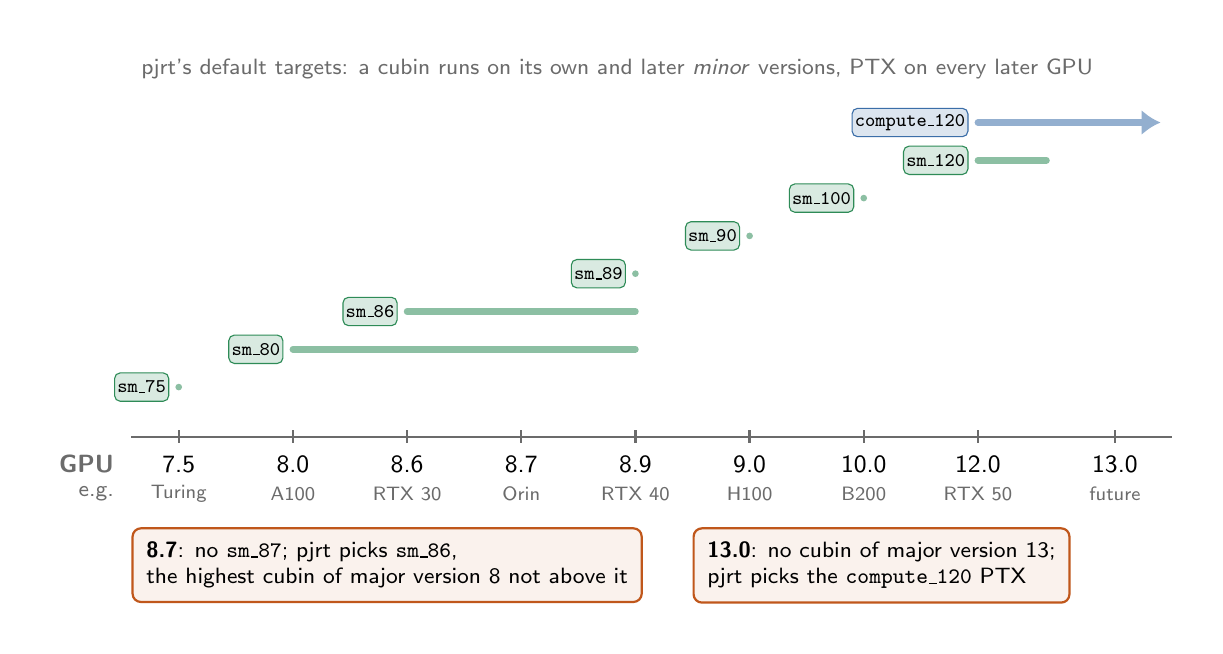
\begin{tikzpicture}[
    arch/.style={font=\sffamily\scriptsize, text=muted},
    img/.style={draw=device, fill=device!18, rounded corners=2pt, minimum height=0.36cm, inner sep=1pt, font=\ttfamily\scriptsize},
    ptximg/.style={img, draw=host, fill=host!18},
    reach/.style={line width=2.4pt, device!55, line cap=round},
    ptxreach/.style={line width=2.4pt, host!55, line cap=round, -{Latex[length=2.4mm, width=3.2mm]}},
  ]
  % GPU architectures on the axis; \pos is the x position
  \def\archs{7.5/0/Turing, 8.0/1/A100, 8.6/2/RTX 30, 8.7/3/Orin, 8.9/4/RTX 40, 9.0/5/H100, 10.0/6/B200, 12.0/7/RTX 50, 13.0/8.2/future}
  \def\dx{1.45}
  \draw[thick, muted] (-0.6, 0) -- ({8.7*\dx}, 0);
  \foreach \cc/\pos/\name in \archs {
    \draw[thick, muted] ({\pos*\dx}, -0.08) -- ({\pos*\dx}, 0.08);
    \node[font=\sffamily\small] at ({\pos*\dx}, -0.35) {\cc};
    \node[arch] at ({\pos*\dx}, -0.72) {\name};
  }
  \node[heading=muted, anchor=east] at (-0.7, -0.35) {GPU};
  \node[note, anchor=east] at (-0.7, -0.72) {e.g.};

  % the shipped images and what they reach
  \foreach \t/\from/\to/\row in {sm\_75/0/0/1, sm\_80/1/4/2, sm\_86/2/4/3, sm\_89/4/4/4, sm\_90/5/5/5, sm\_100/6/6/6, sm\_120/7/7.6/7} {
    \pgfmathsetmacro{\y}{0.15 + 0.48*\row}
    \draw[reach] ({\from*\dx}, \y) -- ({\to*\dx}, \y);
    \node[img, anchor=east] at ({\from*\dx - 0.12}, \y) {\t};
  }
  \pgfmathsetmacro{\y}{0.15 + 0.48*8}
  \draw[ptxreach] ({7*\dx}, \y) -- ({8.6*\dx}, \y);
  \node[ptximg, anchor=east] at ({7*\dx - 0.12}, \y) {compute\_120};

  % worked examples
  \node[accbox, anchor=north west, align=left, font=\sffamily\footnotesize] at (-0.6, -1.15)
    {\textbf{8.7}: no \texttt{sm\_87}; pjrt picks \texttt{sm\_86},\\the highest cubin of major version 8 not above it};
  \node[accbox, anchor=north west, align=left, font=\sffamily\footnotesize] at ({4.5*\dx}, -1.15)
    {\textbf{13.0}: no cubin of major version 13;\\pjrt picks the \texttt{compute\_120} PTX};
  \node[note, anchor=south west, align=left] at (-0.6, {0.15 + 0.48*8.9})
    {pjrt's default targets: a cubin runs on its own and later \emph{minor} versions, PTX on every later GPU};
\end{tikzpicture}
\end{document}
